% -----------------------------------------------
% DCC831 - IA Generativa para Música (UFMG, 2026/2)
% Trabalho Prático 1 - Composição Musical Algorítmica
% Formatado com o template oficial do ISMIR 2026 (github.com/ismir/paper_templates)
% -----------------------------------------------

\documentclass{article}
\usepackage[T1]{fontenc}
\usepackage[utf8]{inputenc}
\usepackage[brazilian]{babel}
\usepackage{ismir} % versão "camera-ready" (sem a opção submission, para exibir o autor)
\usepackage{amsmath,cite,url}
\usepackage{graphicx}
\usepackage{booktabs}
\usepackage{color}

% A nota de copyright do template cita os anais do ISMIR; como este é um trabalho de disciplina, substituímos apenas esse texto
\makeatletter
\renewcommand{\permission}{%
  \begin{figure}[b]{%
    \footnotesize
    {
\includegraphics[alt={CC-BY License},height=0.45cm]{cc_by.pdf}}
    \vskip -.45cm
    \begin{spacing}{1.1}
      \hskip 1.5cm \copyright \hskip .1cm \authorname.
      Licenciado sob Creative Commons Attribution 4.0 International License (CC BY 4.0).
      \textbf{Atribuição:} \authorname,
      ``\removelinebreaks{\@title}'', Trabalho Prático 1 de DCC831 -- IA Generativa para Música, UFMG, 2026.
    \end{spacing}
    }
  \end{figure}
}
% rótulos em português (o ismir.sty os define fixos em inglês)
\def\fnum@figure{\textbf{Figura \thefigure}}
\def\fnum@table{\textbf{Tabela \thetable}}
\def\abstract{\begin{center}\bf RESUMO\end{center}}
\def\thebibliography#1{
  \section{Referências}\list
  {[\arabic{enumi}]}{
  \settowidth\labelwidth{[#1]}\leftmargin 1em
  \advance\leftmargin\labelsep
  \usecounter{enumi}
  }
  \def\newblock{\hskip .01em plus .01em minus .01em}
  \sloppy\clubpenalty4000\widowpenalty4000
  \sfcode`\.=1000\relax
}
\makeatother

\title{Corais à Maneira de Bach com Cadeias de Markov: \\ Novidade versus Memorização}

\oneauthor
  {Pedro Henrique Gonçalves Pires}
  {Departamento de Ciência da Computação -- Universidade Federal de Minas Gerais\\
   \texttt{pedro.pires.edu@gmail.com}}

\def\authorname{P. H. G. Pires}

\sloppy

\begin{document}

\maketitle

\begin{abstract}
Este trabalho apresenta um sistema de composição algorítmica baseado em cadeias de Markov de ordem $n$ que gera melodias de corais no estilo de J.\,S.~Bach, acompanhadas por uma linha de baixo. As probabilidades de transição são aprendidas a partir das linhas de soprano de 117 corais em modo maior do corpus do \texttt{music21}, transpostos para Dó maior. Cada estado codifica altura, duração, posição métrica e presença de fermata. A forma do coral (número fixo de frases terminadas em fermata, com cadência final na tônica) é imposta como restrição durante a amostragem, combinada a \emph{backoff} para ordens menores. Com a variação da ordem $n$ de 1 a 6 e da temperatura de amostragem, foi quantificado o compromisso entre novidade e fidelidade ao corpus: o maior trecho copiado literalmente cresce de 5,6 notas ($n=1$) para 27,8 notas ($n=6$), enquanto a fração de 8-gramas inéditos cai de 100\% para 18\%. A ordem $n=3$ apresentou o melhor equilíbrio entre novidade e idiomatismo.
\end{abstract}

\section{Introdução}\label{sec:introducao}

Cadeias de Markov estão entre os métodos mais antigos de composição algorítmica: a \emph{Illiac Suite} (1957) já usava processos estocásticos para escolher notas~\cite{hiller1959}. Sua atratividade vem da simplicidade: um modelo de ordem $n$ estima a probabilidade da próxima nota dado o contexto das $n$ notas anteriores, e a geração consiste em amostrar repetidamente dessa distribuição.

Neste trabalho foram escolhidas as cadeias de Markov e a \textbf{restrição estilística} de compor \emph{melodias de coral no estilo de Bach}, com forma fixa: $F$ frases (padrão $F=4$), cada uma terminada em fermata, compasso 4/4 e cadência final na tônica. A questão central investigada é o efeito da ordem $n$, que regula o compromisso entre gerar música genérica e reproduzir trechos inteiros do corpus.

\section{Trabalhos Relacionados}\label{sec:relacionados}

Ames~\cite{ames1989} apresenta um tutorial clássico sobre o uso de processos de Markov como modelo composicional, discutindo a escolha da ordem e a construção de matrizes de transição. Conklin~\cite{conklin2003} compara estratégias de amostragem a partir de modelos estatísticos treinados em corpora, incluindo corais de Bach, e aponta que a amostragem aleatória simples tende a gerar trechos de baixa probabilidade global. Pachet e Roy~\cite{pachet2011} mostram como impor restrições (por exemplo, a última nota) a sequências markovianas, ideia adotada aqui de forma simplificada. Os corais de Bach também são um \emph{benchmark} recorrente para modelos neurais, como o DeepBach~\cite{hadjeres2017}.

\section{Método}\label{sec:metodo}

\textbf{Corpus e representação.} Foram usados os corais de Bach do \texttt{music21}~\cite{cuthbert2010}, mantendo peças a quatro vozes em 4/4, sem pausas internas nem quiálteras, com tonalidade estimada maior (117 melodias distintas, 5\,797 notas; o modo menor gera um corpus de 125 peças). Cada peça é transposta para Dó maior pelo menor intervalo possível, preservando a tessitura. A linha de soprano vira uma sequência de estados
$x_t = (h_t, d_t, m_t, f_t)$, onde $h_t$ é a altura em semitons relativa a Dó4, $d_t$ a duração em semínimas, $m_t \in [0,4)$ a posição métrica no compasso e $f_t$ indica fermata. O vocabulário tem 368 estados. Incluir $m_t$ faz o modelo aprender ritmo coerente com o compasso; incluir $f_t$ faz ele aprender onde as frases terminam.

\textbf{Modelo.} A cadeia de ordem $n$ estima, por máxima verossimilhança,
\begin{equation}
P(x_t \mid x_{t-n}^{t-1}) = \frac{C(x_{t-n}^{t-1}, x_t)}{\sum_{x'} C(x_{t-n}^{t-1}, x')},
\end{equation}
onde $C$ são contagens no corpus, com estados especiais de início e fim. Quando o contexto de ordem $n$ não existe (ou todas as continuações são proibidas), o modelo recua para a ordem $n-1$, até a ordem~0 (\emph{backoff}, inspirado em~\cite{katz1987}). A distribuição é reescalada por uma temperatura $T$: $p_i \propto p_i^{1/T}$.

\textbf{Restrições de forma.} A cada passo, são removidos da distribuição os estados que violam: (i) consistência métrica, $m_t = (m_{t-1} + d_{t-1}) \bmod 4$; (ii) frase mínima de 5 notas antes de uma fermata (quinto percentil do corpus); (iii) cadência final: a $F$-ésima fermata deve cair na tônica. A peça termina na $F$-ésima fermata; se ultrapassar $16F$ notas é rejeitada e amostrada novamente.

\textbf{Baixo.} Para tornar a audição mais rica, uma segunda cadeia, condicional, gera o baixo nota a nota: $P(b_t \mid b_{t-1}, h_t, m_t)$, com \emph{backoff} para $P(b_t \mid b_{t-1}, h_t)$, $P(b_t \mid h_t)$, $P(b_t \mid h_t \bmod 12)$ e $P(b_t)$, exigindo baixo pelo menos 3 semitons abaixo do soprano e tônica no último acorde.

\textbf{Hiperparâmetros.} Ordem $n$ (padrão 3), temperatura $T$ (1,0), número de frases $F$ (4), modo (maior/menor) e semente. A saída é MIDI e MusicXML; o áudio (\texttt{.wav}) é sintetizado a partir do MIDI por um sintetizador aditivo simples, só para audição.

\section{Resultados}\label{sec:resultados}

\textbf{Trade-off da ordem.} Foram geradas 30 peças (sementes 0--29) para cada $n \in \{1,\dots,6\}$ e $T \in \{0{,}5;\ 1{,}0;\ 1{,}5\}$, medindo (a)~o maior trecho contíguo da peça idêntico a algum coral do corpus e (b)~a fração de 8-gramas da peça ausentes do corpus (Figura~\ref{fig:tradeoff}). Com $T=1$, o maior trecho copiado cresce de 5,6 ($n=1$) para 14,3 ($n=3$) e 27,8 notas ($n=6$), ou seja, mais da metade de uma peça típica (cerca de 40 notas). A causa é a esparsidade: a fração de contextos com uma única continuação possível sobe de 37\% ($n=1$) para 79\% ($n=3$) e 95\% ($n=6$), de modo que, com $n$ alto, a cadeia apenas ``percorre'' um coral existente. A temperatura tem efeito pequeno perto disso, pois não cria alternativas onde só existe uma.

\begin{figure}[t]
  \centering
  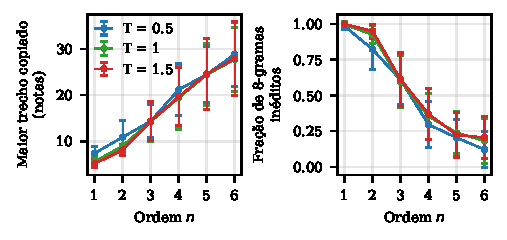
\includegraphics[width=\columnwidth]{../results/tradeoff.pdf}
  \caption{Média e desvio-padrão (30 sementes) do maior trecho copiado do corpus e da fração de 8-gramas inéditos, por ordem $n$ e temperatura $T$.}
  \label{fig:tradeoff}
\end{figure}

\textbf{Peças geradas.} A Tabela~\ref{tab:samples} lista as seis peças entregues no repositório (pasta \texttt{music/}, com \texttt{.mid}, \texttt{.musicxml} e \texttt{.wav}). As duas primeiras usam a mesma configuração com sementes diferentes; as demais variam um hiperparâmetro de cada vez. Na inspeção das partituras, a peça com $n=1$ tem contorno sem direção clara, saltos mais frequentes e uma cadência intermediária cromática (Dó\#--Ré) incomum no estilo, embora termine as frases nos lugares certos graças às restrições. Com $n=3$ as frases têm contorno típico de coral, com passagens em colcheias e cadências idiomáticas (2--1, 7--1 e semicadências 6--5), combinando fragmentos de corais diferentes. Com $n=5$ a melodia é convincente, mas reconhecivelmente colada a um coral real (18 notas seguidas de BWV~69.6). O modo menor com 6 frases mostra que a forma pode ser alterada sem retreinar o modelo. O baixo segue a harmonia implícita na maior parte do tempo, mas cada peça tem até dois pares de quintas ou oitavas paralelas e algumas dissonâncias não preparadas, que o modelo não controla.

\begin{table}[t]
  \centering
  \footnotesize
  \setlength{\tabcolsep}{4pt}
  \begin{tabular}{@{}lccccc@{}}
    \toprule
    Arquivo & $n$ & $T$ & Notas & Cópia & 8-gr. novos \\
    \midrule
    \texttt{major\_o3\_t1\_p4\_s0}   & 3 & 1,0 & 43 & 9  & 89\% \\
    \texttt{major\_o3\_t1\_p4\_s1}   & 3 & 1,0 & 41 & 11 & 71\% \\
    \texttt{major\_o1\_t1\_p4\_s0}   & 1 & 1,0 & 30 & 5  & 100\% \\
    \texttt{major\_o5\_t1\_p4\_s0}   & 5 & 1,0 & 38 & 18 & 39\% \\
    \texttt{major\_o3\_t1.5\_p4\_s0} & 3 & 1,5 & 33 & 14 & 73\% \\
    \texttt{minor\_o3\_t1\_p6\_s0}   & 3 & 1,0 & 47 & 14 & 65\% \\
    \bottomrule
  \end{tabular}
  \caption{Peças entregues. ``Cópia'' é o maior trecho (em notas) idêntico a um coral do corpus. A última peça usa o modo menor e $F=6$ frases.}
  \label{tab:samples}
\end{table}

\section{Discussão e Trabalhos Futuros}\label{sec:discussao}

Os resultados reproduzem o comportamento esperado de cadeias de Markov: ordens baixas são mais aleatórias e genéricas, ordens altas são fiéis ao corpus mas memorizam trechos inteiros, porque o corpus (cerca de 5,8 mil notas) é pequeno para o número de contextos possíveis. A ordem $n=3$ foi escolhida como padrão porque é o ponto em que a maioria dos 8-gramas ainda é inédita (60\%), mas as frases já soam idiomáticas. As restrições de forma se mostraram essenciais: sem elas, a cadeia não controla o número nem o tamanho das frases.

Entre as limitações estão a falta de estrutura de longo prazo (não há repetição de motivos entre frases), a harmonia apenas implícita no baixo e a avaliação qualitativa feita apenas pelo autor, sem teste de audição. Como extensões, são propostas: suavização mais robusta (\emph{interpolated Kneser--Ney}); a imposição de restrições pelo método de Pachet e Roy~\cite{pachet2011}, que preserva as probabilidades da cadeia em vez de apenas filtrar estados; a geração das quatro vozes com uma cadeia sobre acordes; e um teste de audição com outros ouvintes.

\bibliography{ISMIRtemplate}

\end{document}
